\documentclass[12pt]{book}

%These tell TeX which packages to use.
\usepackage{array,epsfig}
\usepackage{amsmath}
\usepackage{amsfonts}
\usepackage{amssymb}
\usepackage{amsxtra}
\usepackage{amsthm}
\usepackage{mathrsfs}
\usepackage{color}
\usepackage{enumitem}
%\usepackage{mdframed}
\usepackage[most]{tcolorbox}
\usepackage{pgfplots}
\pgfplotsset{compat=1.6}

\pgfplotsset{soldot/.style={color=black,only marks,mark=*}} \pgfplotsset{holdot/.style={color=black,fill=white,only marks,mark=*}}

%Here I define some theorem styles and shortcut commands for symbols I use often
\theoremstyle{definition}
\newtheorem{defn}{Definition}
\newtheorem{thm}{Theorem}
\newtheorem{cor}{Corollary}
\newtheorem*{rmk}{Remark}
\newtheorem{lem}{Lemma}
\newtheorem*{joke}{Joke}
\newtheorem{ex}{Example}
\newtheorem*{soln}{Solution}
\newtheorem{prop}{Proposition}

\newcommand{\lra}{\longrightarrow}
\newcommand{\ra}{\rightarrow}
\newcommand{\surj}{\twoheadrightarrow}
\newcommand{\graph}{\mathrm{graph}}
\newcommand{\bb}[1]{\mathbb{#1}}
\newcommand{\Z}{\bb{Z}}
\newcommand{\Q}{\bb{Q}}
\newcommand{\R}{\bb{R}}
\newcommand{\C}{\bb{C}}
\newcommand{\N}{\bb{N}}
\newcommand{\M}{\mathbf{M}}
\newcommand{\m}{\mathbf{m}}
\newcommand{\MM}{\mathscr{M}}
\newcommand{\HH}{\mathscr{H}}
\newcommand{\Om}{\Omega}
\newcommand{\Ho}{\in\HH(\Om)}
\newcommand{\bd}{\partial}
\newcommand{\del}{\partial}
\newcommand{\bardel}{\overline\partial}
\newcommand{\textdf}[1]{\textbf{\textsf{#1}}\index{#1}}
\newcommand{\img}{\mathrm{img}}
\newcommand{\ip}[2]{\left\langle{#1},{#2}\right\rangle}
\newcommand{\inter}[1]{\mathrm{int}{#1}}
\newcommand{\exter}[1]{\mathrm{ext}{#1}}
\newcommand{\cl}[1]{\mathrm{cl}{#1}}
\newcommand{\ds}{\displaystyle}
\newcommand{\vol}{\mathrm{vol}}
\newcommand{\cnt}{\mathrm{ct}}
\newcommand{\osc}{\mathrm{osc}}
\newcommand{\LL}{\mathbf{L}}
\newcommand{\UU}{\mathbf{U}}
\newcommand{\support}{\mathrm{support}}
\newcommand{\AND}{\;\wedge\;}
\newcommand{\OR}{\;\vee\;}
\newcommand{\Oset}{\varnothing}
\newcommand{\st}{\ni}
\newcommand{\wh}{\widehat}
%Pagination stuff.
\setlength{\topmargin}{-0.75in}
\setlength{\oddsidemargin}{0in}
\setlength{\evensidemargin}{0in}
\setlength{\textheight}{9.in}
\setlength{\textwidth}{6.5in}
\pagestyle{empty}
\begin{document}
\begin{flushleft}
Name:\underline{\hspace{13cm}}Date:\underline{\hspace{2cm}}
\end{flushleft}
\begin{center}
{\Large Math 1041-012 \hspace{0.5cm} Section 3.5: Implicit Differentiation}
\end{center}
%\vspace{0.2 cm}
\subsection*{Motivating Example}
How do we find the derivative $y'$ when a function is given as
\[
x^2+y^2=25
\]
This is called \textit{implicitly defined} function.
\begin{tcolorbox}
\subsection*{Implicit Differentiation Process}
\begin{itemize}
    \item[(1)] Find the derivatives with respect to $x$ and $y$ variables on both sides of the equal sign.
    \item[(2)] Wherever you took the derivative of $y$ multiply by $y'$
    \item[(3)] If possible solve (isolate) for the $y'$ so that your final answer reads
    \[
    y'=...blah...blah...
    \]
\end{itemize}
\end{tcolorbox}
\subsubsection*{Step-by-Step Example}
If $x^2+y^2=25$ find $\frac{dy}{dx}$. Then find the equation of the tangent line at $x=3$.
\raggedbottom
\clearpage
\subsection*{Example: folium of Descartes}
\begin{itemize}
    \item[(a)] Find $y'$ if $x^3+y^3=6xy$
    \item[(b)] Find the equation of the tangent line at $x=3$.
    \item[(c)] At what point in the first quadrant is the tangent horizontal??
\end{itemize}
\vspace{7cm}
\subsection*{Example: Why can't we do regular derivatives?}
Find $y'$ given $\sin(x+y)=y^2\cos x$. Is is possible to isolate the $y$??
\raggedbottom
\clearpage
\subsection*{Example: Higher Derivatives}
Find $y''$ if $x^4+y^4=16$.\vspace{7cm}
\subsection*{Implicit Differentiation to find Derivatives of inverse trig functions}
What is
\[
\frac{d}{dx}\sin^{-1}x=??
\]
Follow the process:
\raggedbottom
\clearpage
\subsection*{You try!}
\begin{itemize}
\item[(a)]Find $y'$ if $y=\cos^{-1}x$ \vspace{6cm}
\item[(b)]Find $y'$ if $y=\tan^{-1}x$\vspace{4cm}
\end{itemize}
\begin{figure}[h!]
    \centering
    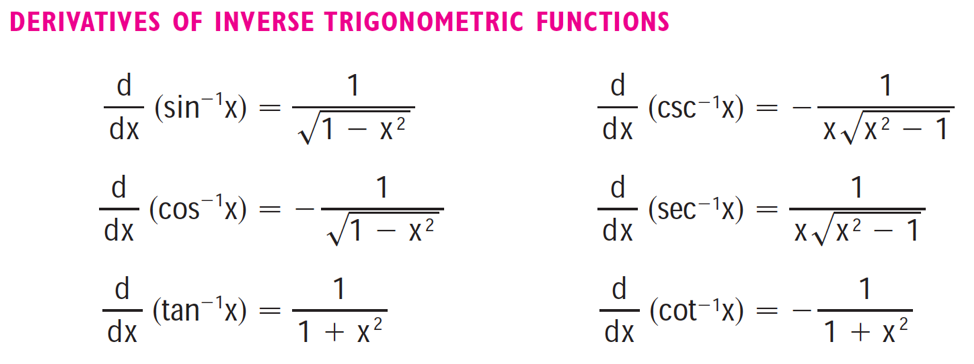
\includegraphics{fig2.png}
\end{figure}
\end{document}